\documentclass[../main.tex]{subfiles}

\begin{document}

As mentioned in Section \ref{sec:results}, EngSci Press generally meets my expectation. However, more objectives emerged as I worked on this project, which might serve as a guide for future work.

\begin{enumerate}
	\item \textit{Unicode support.}
	Many users look up words in a different language, so it is hard to avoid non-ASCII characters. Unfortunately, this need has not yet been satisfied as because of the limited Unicode support \cite{bib:c_unicode} in C standard library (especially IO). Porting from \texttt{char} to \texttt{wchar\_t} \cite{bib:wchar_t}, the most common approach, can cause a memory disaster, quadrupling the current 300MB to 1.2GB. I prefer variable-width encoding because it is more efficient in terms of memory. It is messy to implement and might require 3rd-party wheels.
	
	\item \textit{Compact trie (or radix tree).}
	Currently, a trie node can hold one character at most. However, it will be appealing to put multiple characters together if a group of adjacent nodes have only one child for each, as shown in Figure \ref{fig:compact_trie}. It certainly saves memory. On the other hand, it might also run faster because of smaller tree heights.
	
	\item \textit{Gammatical agreement.}
	This phenomenon is common in a natural language (e.g.\ 3rd-person-singular verbs), but painful to describe in CFG. For example, ``do'' can be transformed to ``does'', ``do'', ``did'', ``has done'', ``have done'', ``am doing'', ``is doing'', ``are doing'', given different nouns, pronouns, and tenses. As a result, a rule on ``do'' has to repeat itself for each of the versions. Making tokens contain parameters (or variables) \cite{bib:context_free_grammar} can free human labour from this process. As shown in Figure \ref{fig:template_rule}, parametrized rules can serve as templates to generate many rules with normal tokens.
\end{enumerate}

\begin{figure}
	\centering
	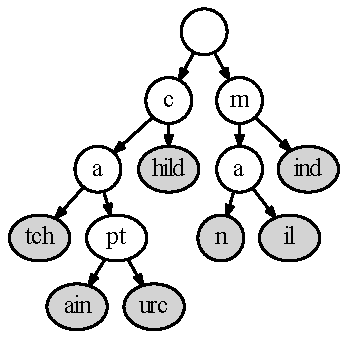
\includegraphics{compact_trie}
	\caption{Compact version of the trie in Figure \ref{fig:trie}. Each shadowed node holds one or more English words.}
	\label{fig:compact_trie}
\end{figure}

\begin{figure}
	\begin{equation*}
	\begin{aligned}
	& \text{S} \mapsto \text{NP-Singular} \; \text{VP-Singular} \\
	& \text{S} \mapsto \text{NP-Plural} \; \text{VP-Plural} \\
	& \text{S} \mapsto \text{NP-Singular} \; \text{VP-Singular} \; \text{NP-Singular} \\
	& \text{S} \mapsto \text{NP-Singular} \; \text{VP-Singular} \; \text{NP-Plural} \\
	& \text{S} \mapsto \text{NP-Plural} \; \text{VP-Plural} \; \text{NP-Singular} \\
	& \text{S} \mapsto \text{NP-Plural} \; \text{VP-Plural} \; \text{NP-Plural}
	\end{aligned}
	\; \Longleftrightarrow \;
	\text{S} \langle T \rangle \mapsto \text{NP}\langle T \rangle \; \text{VP} \langle T \rangle \; (\text{NP} \langle U \rangle )
	\end{equation*}
	\caption{Template rules make it easier to describe grammatical agreements.}
	\label{fig:template_rule}
\end{figure}

\end{document}